% !TeX spellcheck = en_US
\section{Overall system architecture and services}
\begin{itemize}
	\item cf. \ref{fig:system-overview}
	\item \todo{highlight the differences between optimal (proposed) infrastructure and the implementation}
\end{itemize}

\begin{figure}[h]
	\centering
	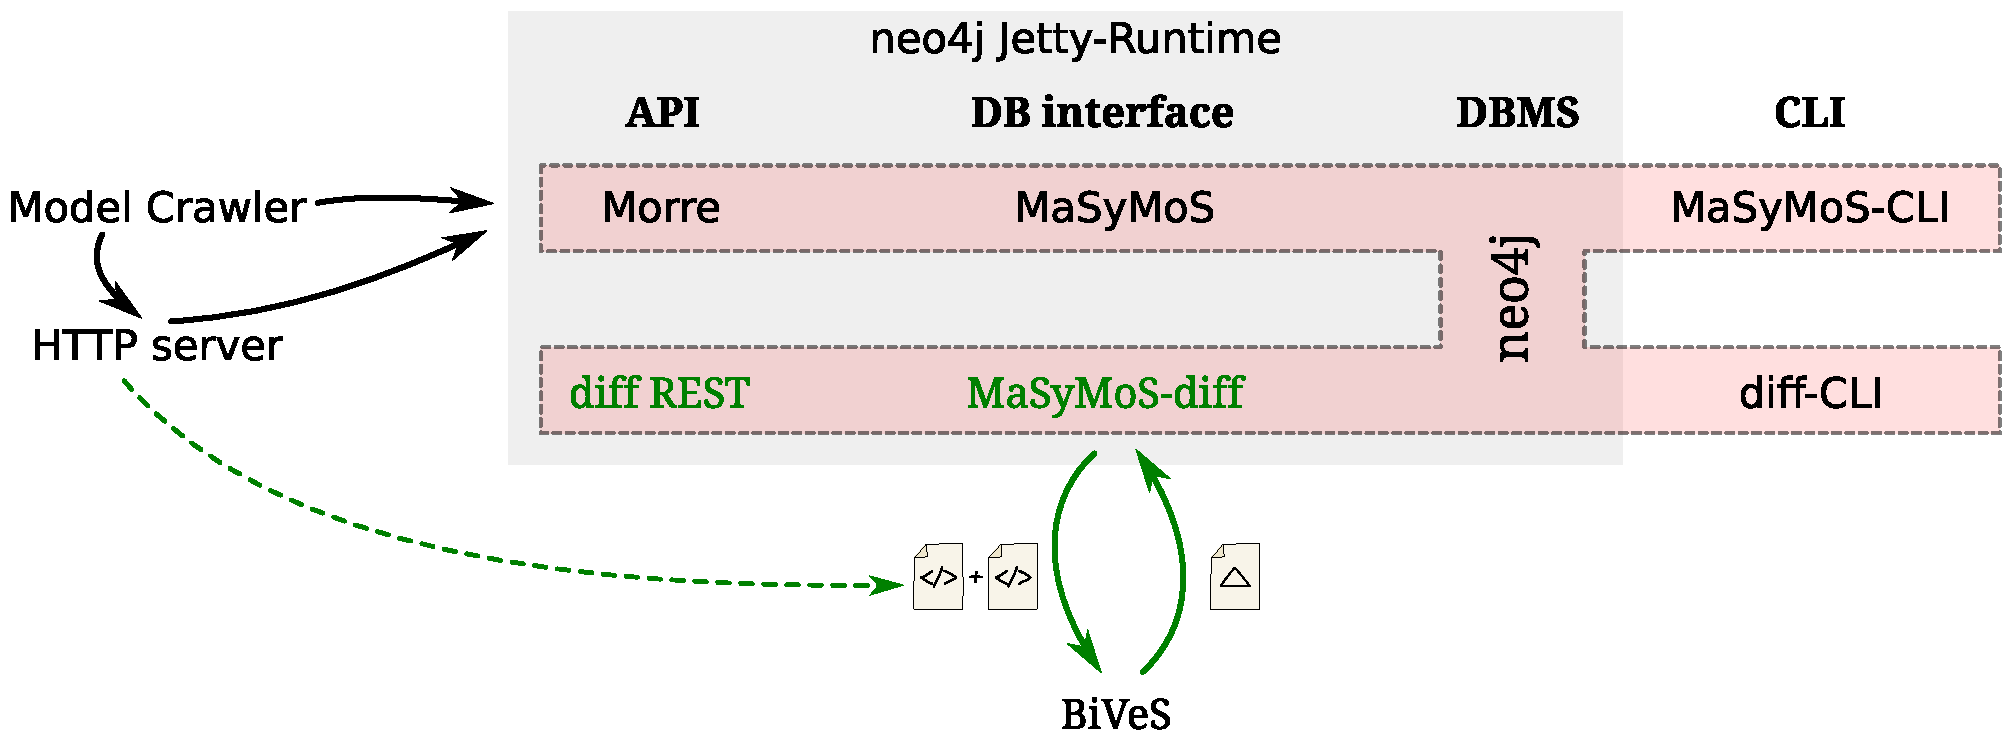
\includegraphics[width=\textwidth]{resources/system-overview-matrix.pdf}
	\caption{Infrastructure overview}
	\label{fig:system-overview}
\end{figure}

\section{Database model and storage decisions}
\begin{itemize}
\item extension to database model cf. \ref{fig:db-model}
	\subitem linking version
	\subitem storing differences
\item decisions on storage model
	\subitem storing each version full (no delta-storage)
	\subitem each version is aware to the search index
	\subitem diff still enables for analysis of changes
	\subitem higher storage consumption
\item extended storage model
\end{itemize}
% description of ER model
Figure \ref{fig:db-er-model} shows the proposed database schema as ER model. To reduce complexity and redundancy, the storage structure of models in \masymos is simplified, shown on the left hand side of the figure. Further the \comodi ontology (cf. Section \ref{sec:background:onto:comodi}) is not remodeled, but instead represented as generic \texttt{OntologyTerm}.

\todo{Add color to the diagram, to ease explanation}
\todo{Find out, to what a Diff can link}

The schema is organized around a \texttt{Diff} entity linking two \texttt{Document} entities, which represent an (XML-)document containing a model. The interlink is expressed via the \texttt{has\_diff} relation, which can be expressed in two roles: \texttt{source} and \texttt{destination}. I decided to use these terms in order to prevent confusion regarding the time line of the model versions, since \bives also does not discriminate any temporal information.
This 2-hop relation does not necessarily need to span between two consecutive versions, but I decided for a standard setup it might be less useful to store differences between every possible combination of versions, since it would consume unreasonable amount of storage. Further are deltas concatable, so it does not take any significant computational effort to generate a diff for larger version steps out of consecutive diffs.

Every \texttt{Diff} entity links to one or multiple \texttt{DiffEntry} via the \texttt{has\_entry} relation.  
A \texttt{DiffEntry} can be either a \texttt{DiffInsert},  \texttt{DiffDelete}, \texttt{DiffMove} or a \texttt{DiffUpdate} entity, following the terms used by \bives \cite{Scharm2015} and \comodi \cite{Scharm2016}.

Each \texttt{DiffEntry} represents a difference detected by \bives \cite{Scharm2015} and links to at least on \texttt{ModelEntity} via either \texttt{is\_source}, a \texttt{is\_destination}, or both, depending on the type of the difference.
For instance a \texttt{DiffInsert} links to a \texttt{ModelEntity} of the \emph{destination} with a \texttt{is\_destination} relation.
In contrast a \texttt{DiffDelete} links to the \emph{source} version with \texttt{is\_source} to a \texttt{ModelEntity}. Whereby \texttt{DiffMove} and \texttt{DiffModify} use both relations \texttt{is\_source} - linking to the \emph{source} - and \texttt{is\_destination} - linking to the \emph{destination} version.

Additionally a \texttt{DiffEntry} can link to an \texttt{OntologyTerm}, which again are hierarchical structured, but not modeled in this ER model. Those terms are currently only taken from the \comodi ontology \cite{Scharm2016}, cf. Section \ref{sec:background:onto:comodi}, since no other ontology exists, describing changes.

\todo{add table (or similar) of all entities and relations in the appendix}
\todo{make visible, that ER model is just a sub-ER}

This storage structure, I decided on, does not make use of efficient reverse-delta storage, as traditional VCS (cf. Section \ref{sec:background:manage-versions:traditional-vcs}), instead each model is stored complete for multiple reasons: It allows for a very lose coupling to the base \masymos implement ion, means the diff-extension is additive to the features of \masymos and does not require for intrusive changes of the code base. Further the core functionality of \masymos, providing a full text and structural search index, is not disturbed, so if required each version of a model can be treated as single instance. Resulting in easier structural analyses per model version and less expensive operations on the indexes, when inserting a new model version.

On the other hand the complete storage of each model increases the database size significantly. But to keep the scope of this work concise and the implementation reasonable, I focused on a good data interlinkage and less on a storage efficient data model. \todo{revise?}
\begin{figure}
	\centering
	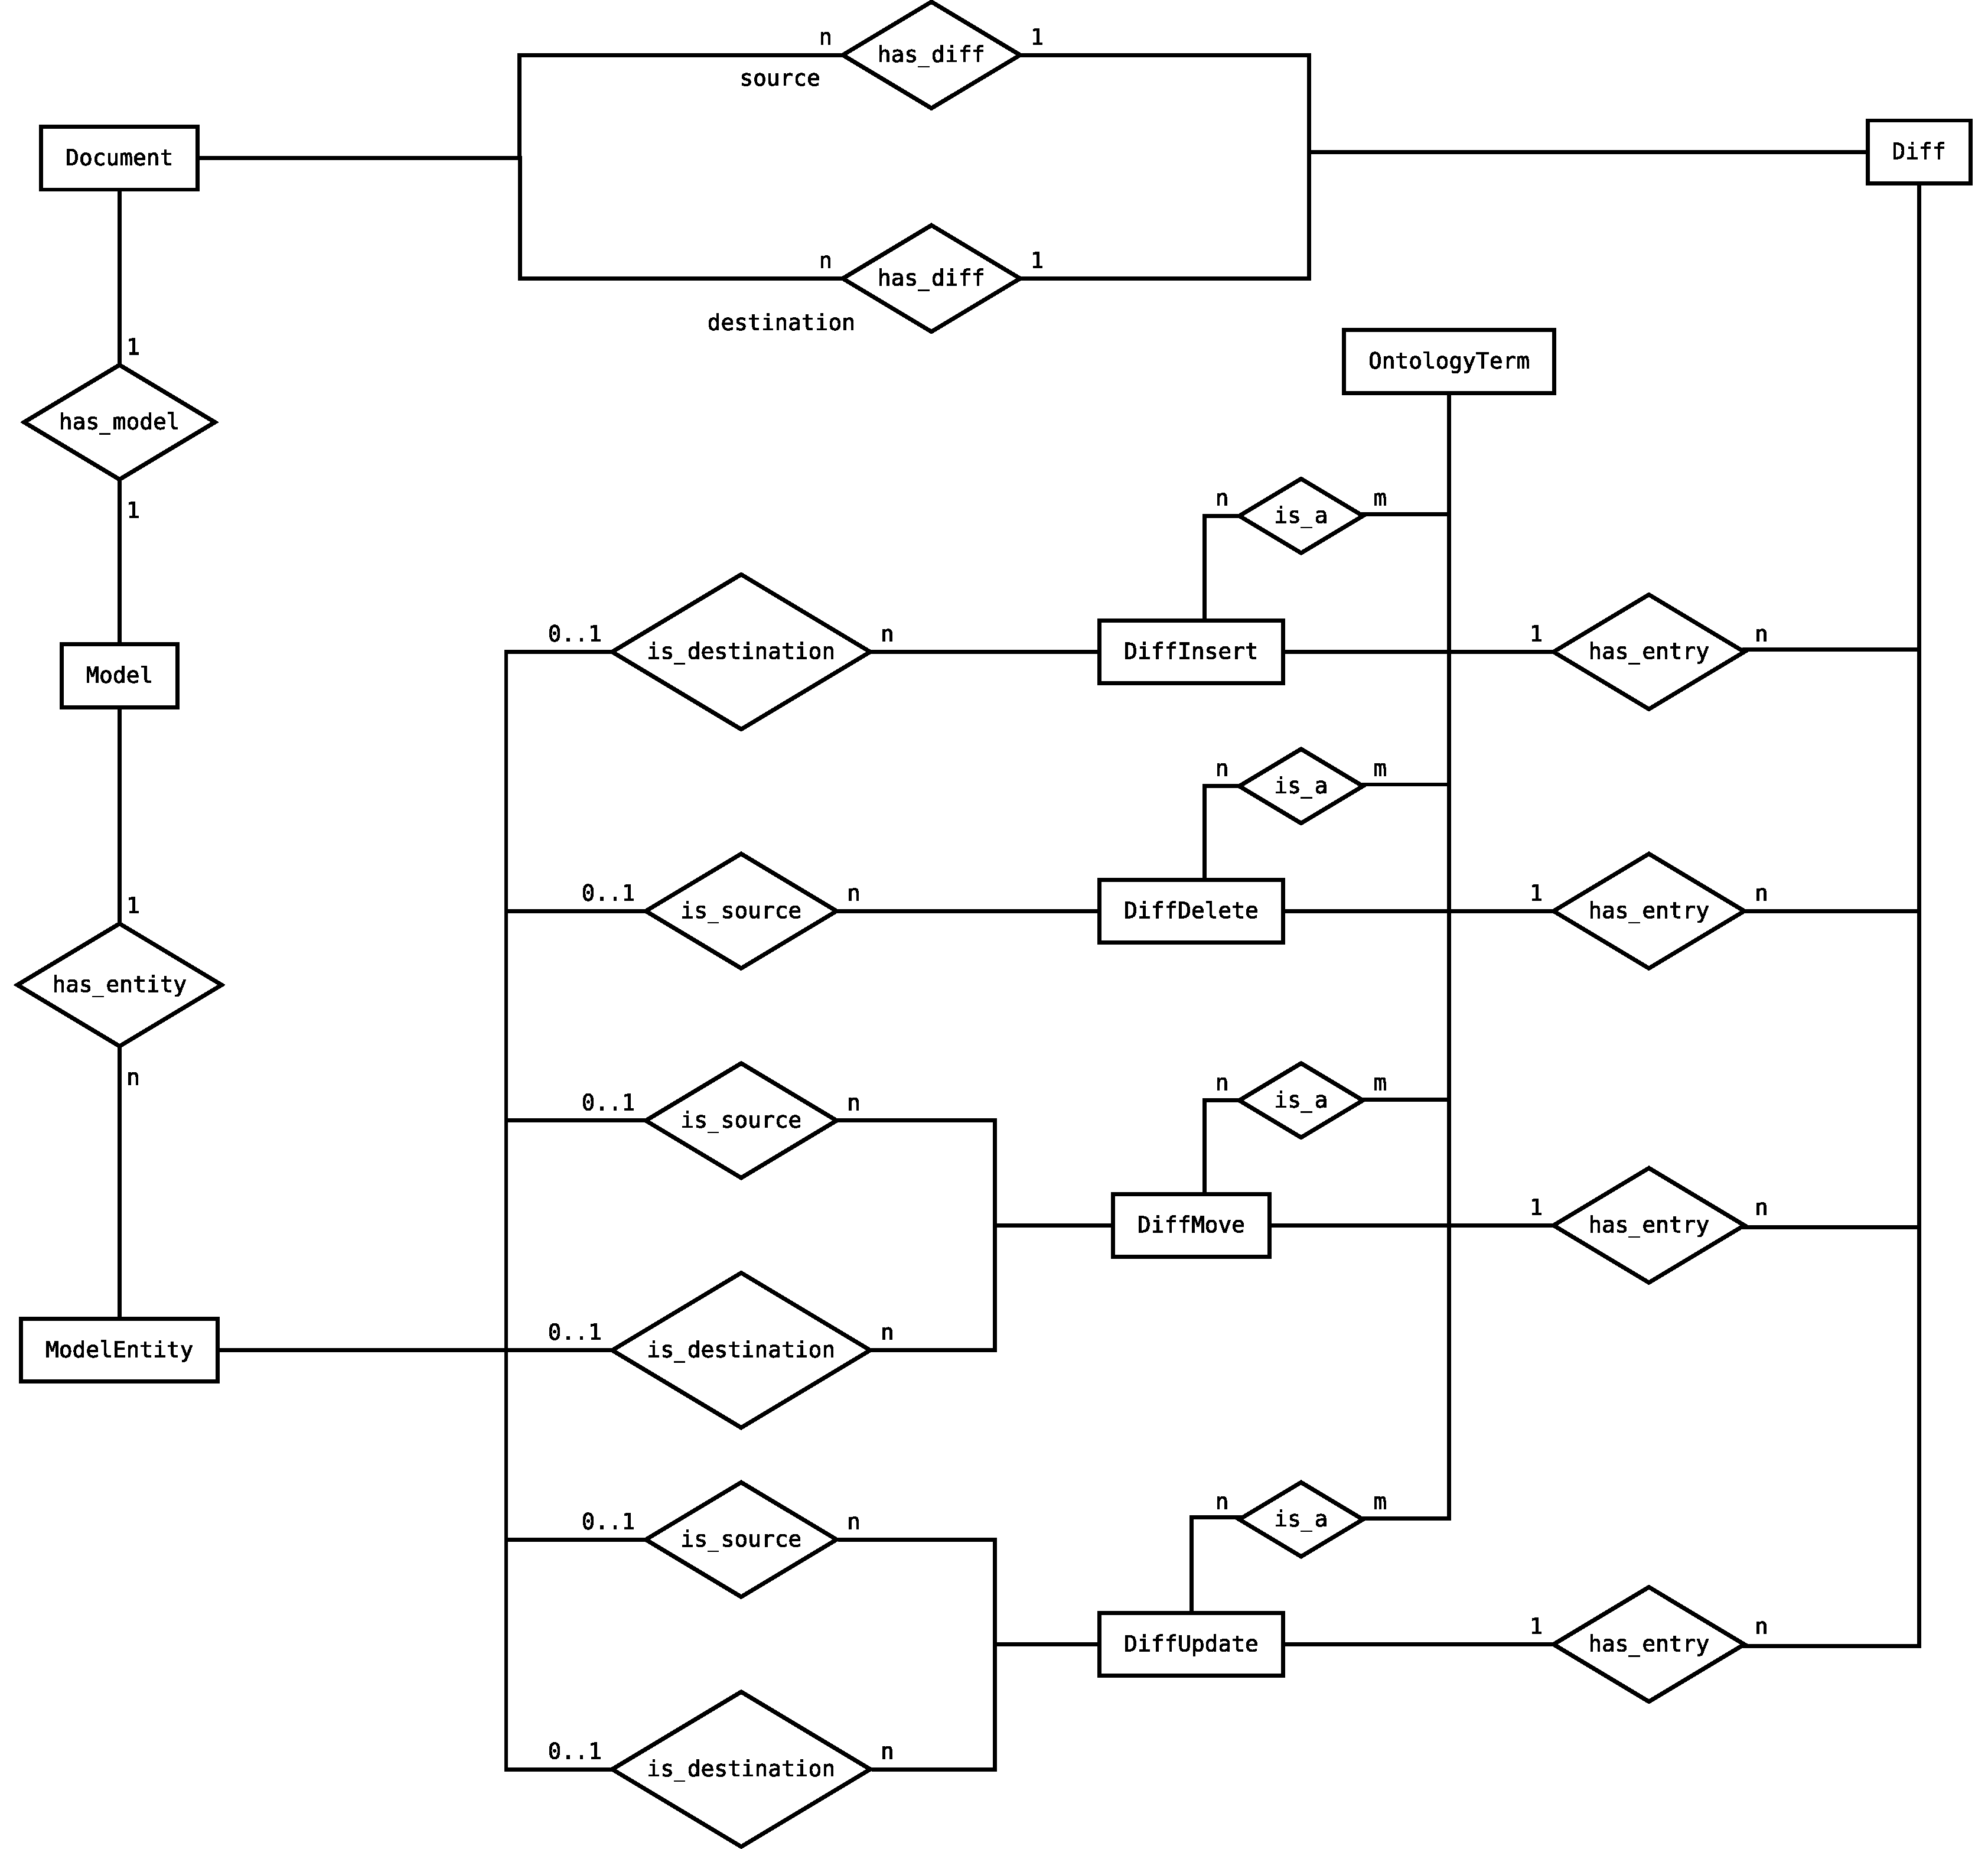
\includegraphics[width=\textwidth]{resources/db-concept-er.pdf}
	\caption{ER model of the proposed database schema}
	\label{fig:db-er-model}
\end{figure}

\begin{figure}[h]
	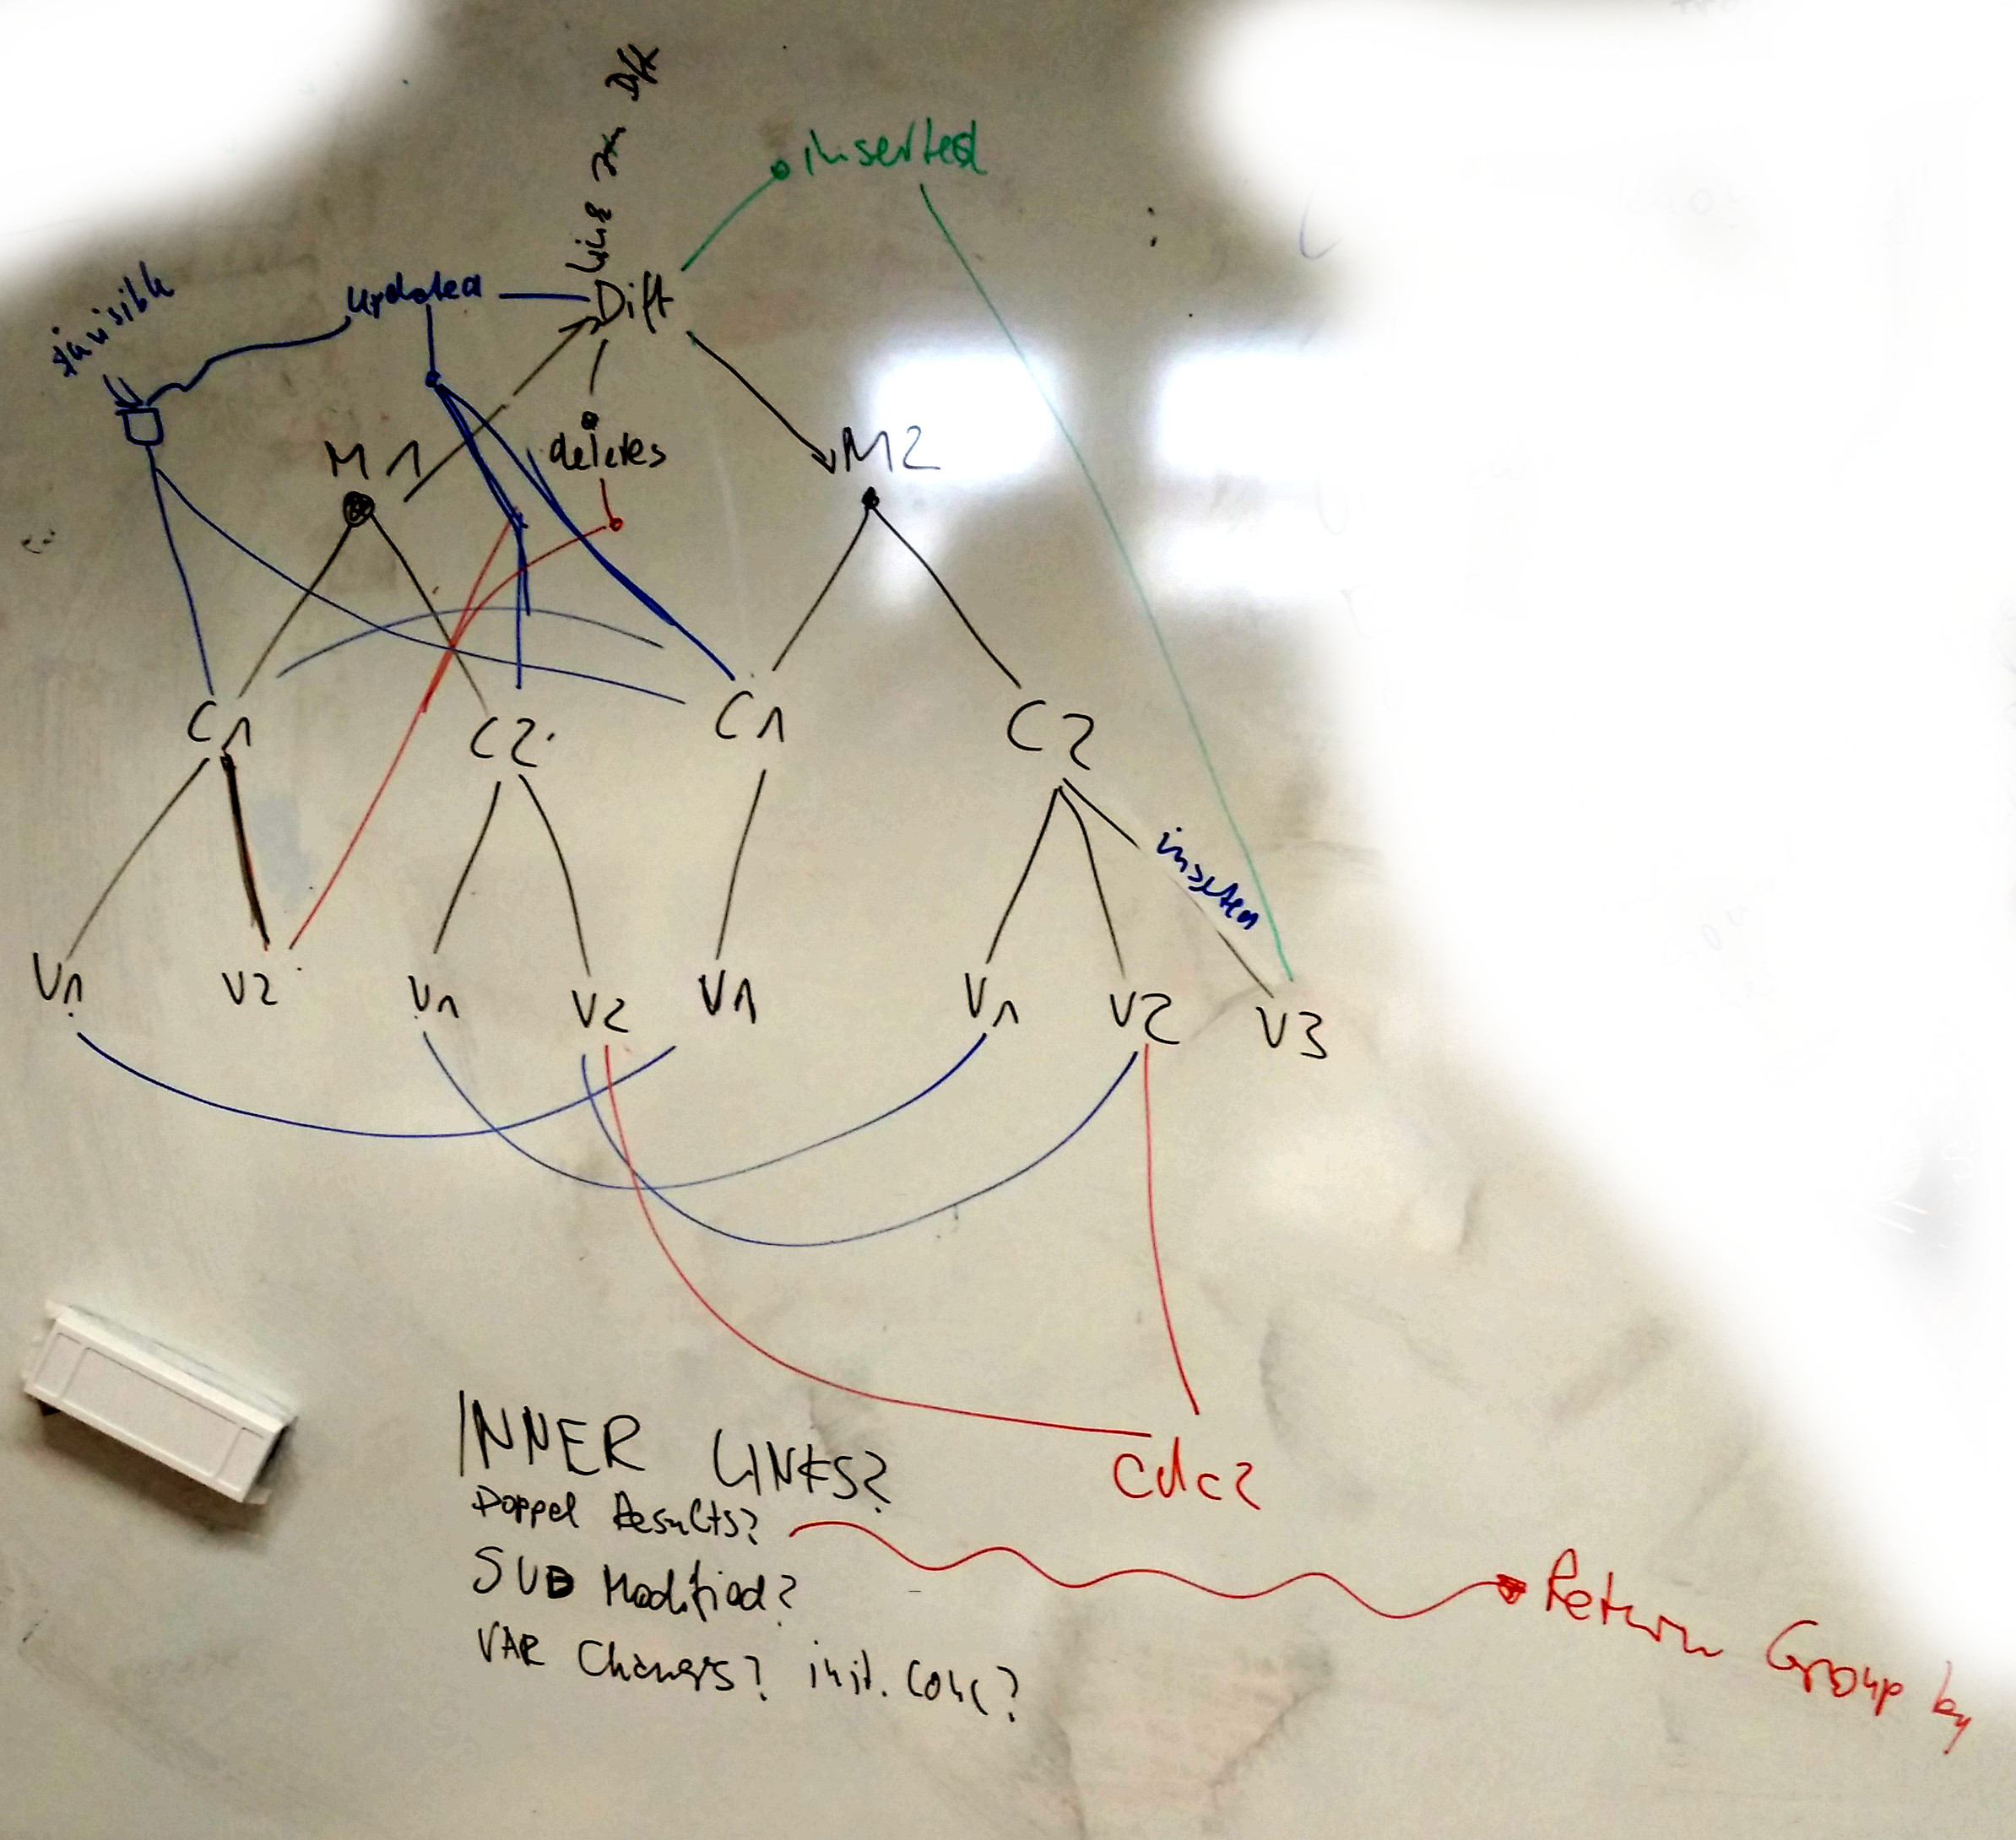
\includegraphics[width=\textwidth]{resources/db_structure.jpg}
	\caption{Proposed database structure}
	\label{fig:db-model}
\end{figure}
